\chapter{Nonlinear governing equation for large transverse displacement}

\section{Additional geometric details}

The curvature, $\kappa$, is defined as
\begin{align*}
\kappa = \pdv{\theta}{s}
\end{align*}
where $\theta$ is the angle between the position of the pipe and the $x_0$-axis while $s$ is the curvilinear coordinate along the pipe. 
As the centerline of the cantilevered pipe is assumed to be inextensible, we also have the following in terms of $x_0$-coordinate
\begin{align*}
\kappa = \pdv{\theta}{s} = \pdv{\theta}{x_0}
\end{align*}
Now,
\begin{align*}
\cos(\theta) = \pdv{x}{s} = \left(1 + \pdv{u}{s}\right)&,~\sin(\theta) = \pdv{z}{s} =\pdv{w}{s}  \\
\tan(\theta) = \frac{\sin (\theta)}{\cos(\theta)} &, \implies~\theta = \tan^{-1}\left(\frac{\pdv{z}{s}}{\pdv{x}{s}}\right)
\end{align*}
Now, curvature is given as
\begin{align*}
\kappa &= \frac{1}{1 + \left(\frac{\pdv{z}{s}}{\pdv{x}{s}}\right)^2}\frac{\pdv[2]{z}{s}\pdv{x}{s} - \pdv{z}{s}\pdv[2]{x}{s}}{(\pdv{x}{s})^2} \\
&= \frac{\pdv[2]{z}{s}\pdv{x}{s} - \pdv{z}{s}\pdv[2]{x}{s}}{(\pdv{x}{s})^2 + (\pdv{z}{s})^2} \\
&=  \pdv[2]{z}{s}\pdv{x}{s} - \pdv{z}{s}\pdv[2]{x}{s}  \qquad (\text{using eqn \ref{eqn:inextensibility}})
\end{align*}
Further simplification gives us
\begin{align}
\kappa &= \frac{\pdv[2]{z}{s}}{\sqrt{1 - (\pdv{z}{s})^2}} \label{eqn:curvature}
\end{align}

\section{Derivation of the equation of motion}
Let us redefine the Lagrangian of the system, $\mathcal{L}$ (drop the subscript $o$) in eqn \ref{eqn:Lo} as
\begin{align*}
 \mathcal{L} = T_f + T_p - V_f - V_p
\end{align*}
where $T_p$ and $V_p$ are the kinetic and potential energies associated with the pipe, while $T_f$ and $V_f$ are the corresponding quantities of the enclosed fluid.

\paragraph{Kinetic energy of the system} The total kinetic energy of the system is 
\begin{align}
   T = T_p + T_f = \frac{1}{2}m \int_0^L V_p^2 ds + \frac{1}{2}M \int_0^L V_f^2 ds
\end{align}
where $m$ and $M$ are the linear mass densities of the pipe and the fluid while $V_p$ and $V_f$ are the velocities of a pipe element and a fluid element.

Let us consider a small segment of pipe and fluid (see fig \ref{fig:coordinate-system-pipe}). By definition, velocity of the pipe element is
\begin{align*}
   \vb{V}_p = \pdv{\vb{r}}{t} = \dot{x}\vb{i} + \dot{z}\vb{k}
\end{align*}
Velocity of the fluid element is 
\begin{align*}
 \vb{V}_f = \vb{V}_p + U \vb{\tau}
\end{align*}
where $\vb{\tau}$ is the tangential unit vector, $\vb{\tau} = \pdv{x}{s} \vb{i} + \pdv{z}{s}\vb{k}$. And so, 
\begin{align*}
\vb{V}_f = \dot{x}\vb{i} + \dot{z}\vb{k} + U\left(\pdv{x}{s} \vb{i} + \pdv{z}{s}\vb{k}\right) = \left(\pdv{}{t} + U\pdv{}{s}\right)(x\vb{i} + z\vb{k}) \equiv \frac{D\vb{r}}{Dt}
\end{align*}
Now, 
\begin{align}
T = \frac{1}{2}m \int_0^L (\dot{x}^2 + \dot{z}^2) ds + \frac{1}{2}M \int_0^L [(\dot{x} + Ux')^2 + (\dot{z} + Uz')^2] ds \label{eqn:total-kinetic-energy}
\end{align}
where prime ($'$) indicates differentiation with respect to $s$.

\paragraph{Potential energy of the system} Potential energy comprises of gravitational energy and strain energy components.

In general, gravitational energy of a mass of density $\rho$ immersed in a uniform gravitational field of strength $g$ is given by $G = -\int_\mathcal{V} \rho\vb{g} \cdot \vb{\xi}d\mathcal{V}$, where $\vb{\xi}$ is the position vector of a mass element with respect to some origin.

Here, gravitational energy of the pipe-fluid system is
\begin{align}
 G = - (m + M)g\int_0^L x ds \label{eqn:gravitational-energy}
\end{align}
The strain energy is given by 
\begin{align}
  V = \frac{1}{2} \int_0^L EI \kappa^2 ds \label{eqn:strain-energy}
\end{align}
where $E$ is the Young's modulus, $I$ is the moment of inertia and $\kappa$ is the curvature.	

\subsection{Variational operations}
Let us apply the variational operation on the expression for the total kinetic energy (eqn \ref{eqn:total-kinetic-energy}) as

\begin{align*}
   \delta \int_{t_1}^{t_2} T~dt & = m \int_{t_1}^{t_2} \int_0^L (\dot{x}\delta \dot{x} + \dot{z}\delta \dot{z})~ds~dt + M \int_{t_1}^{t_2} \int_0^L [(\dot{x} + Ux')(\delta \dot{x} + U\delta x') + (\dot{z} + Uz')(\delta \dot{z} + U\delta z')]~ds~dt \\
     &= m \int_{t_1}^{t_2} \int_0^L (\dot{x}\delta \dot{x} + \dot{z}\delta \dot{z})~ds~dt + M \int_{t_1}^{t_2} \int_0^L [\dot{x}\delta \dot{x} + U \dot{x}\delta x' + Ux'\delta \dot{x} +U^2x'\delta x'  \\ 
     &\phantom{=} \qquad\qquad\qquad\qquad\qquad\qquad\qquad\qquad\qquad + \dot{z}\delta \dot{z} + U \dot{z}\delta z' + Uz'\delta \dot{z} +U^2z'\delta z']~ds~dt  \\
     &= m \int_{t_1}^{t_2} \int_0^L (\dot{x}\delta \dot{x} + \dot{z}\delta \dot{z})~ds~dt + M \int_{t_1}^{t_2} \int_0^L [\dot{x}\delta \dot{x}+ \dot{z}\delta \dot{z} + U \dot{x}\delta x' + U \dot{z}\delta z' + Ux'\delta \dot{x} + Uz'\delta \dot{z} \\
     &\phantom{=} \qquad\qquad\qquad\qquad\qquad\qquad\qquad\qquad\qquad + U^2 \underbrace{(x'\delta x' + U^2z'\delta z')}_{=0~\text{(from inextensibility condition)}}]~ds~dt  \\
     &= \int_{t_1}^{t_2} \int_0^L[(m + M) \dot{x}\delta \dot{x} + (m + M) \dot{z}\delta \dot{z} + M (U \dot{x}\delta x' + U \dot{z}\delta z') + M (Ux'\delta \dot{x} + Uz'\delta \dot{z})]~ds~dt\\
\end{align*}

Integrating by parts the terms on the right hand side and using the following conditions
\begin{itemize}
	\item Zero variations at $t_1$ and $t_2$: $\delta x = \delta z = 0$
	\item Boundary constraint at $s= 0$: $\delta x= \delta z = 0$
\end{itemize} 

Now, 

\begin{align*}
\delta \int_{t_1}^{t_2} T~dt & = \int_0^L \left[(m + M)\dot{x}\delta x\bigg|_{t_1}^{t_2} - \int_{t_1}^{t_2}  (m + M) \ddot{x}\delta x dt + (m + M)\dot{z}\delta z\bigg|_{t_1}^{t_2} - \int_{t_1}^{t_2}  (m + M) \ddot{z}\delta z dt \right]ds \\
   &\phantom{=}~ + \int_{t_1}^{t_2} \left[MU\dot{x}\delta x\bigg|_0^L + MU\dot{z}\delta z\bigg|_0^L - \int_0^L M (U\dot{x}'\delta x + U\dot{z}'\delta z)~ds\right]~dt \\
    &\phantom{=}~ + \int_0^L \left[MUx'\delta x\bigg|_{t_1}^{t_2} + MUz'\delta z\bigg|_{t_1}^{t_2} - \int_{t_1}^{t_2} M(\dot{(Ux')}\delta x  + \dot{(Uz')}\delta z)~dt\right]~ds \\
    & = - \int_0^L \left[\int_{t_1}^{t_2}  (m + M) \ddot{x}\delta x dt + \int_{t_1}^{t_2}  (m + M) \ddot{z}\delta z dt \right]ds \\
    &\phantom{=}~ + \int_{t_1}^{t_2} \left[MU\dot{x}_L\delta x_L + MU\dot{z}_L\delta z_L - \int_0^L M (U\dot{x}'\delta x + U\dot{z}'\delta z)~ds\right]~dt \\
    &\phantom{=}~ - \int_0^L \left[\int_{t_1}^{t_2} M((\dot{U}x' + U\dot{x}')\delta x  + (\dot{U}z' + U\dot{z}')\delta z)~dt\right]~ds \\
    & = - \int_{t_1}^{t_2}\int_0^L \left[  (m + M) \ddot{x} + M\dot{U}x' + 2M U\dot{x}'\right]\delta x~ds~dt \\
    &\phantom{=}~ - \int_{t_1}^{t_2}\int_0^L \left[  (m + M) \ddot{z} + M\dot{U}z' + 2M U\dot{z}'\right]\delta z~ds~dt\\
    &\phantom{=}~ + MU \int_{t_1}^{t_2} (\dot{x}_L\delta x_L + \dot{z}_L\delta z_L)~dt
\end{align*}
where $x_L = x (s = L)$ and $z_L = z (s = L)$ \\
Now, we apply variational operation to the strain energy (eqn \ref{eqn:strain-energy})
\begin{align*}
\delta \int_{t_1}^{t_2} V~dt  = \frac{1}{2}  EI \int_{t_1}^{t_2} \int_0^L\kappa^2~ ds~dt 
\end{align*}
Let us approximate curvature (assuming small transverse displacement)  from eqn \ref{eqn:curvature} as
\begin{align*}
  \kappa^2 = \frac{(\pdv[2]{z}{s})^2}{1 - (\pdv{z}{s})^2} \approx \left(\pdv[2]{z}{s}\right)^2\left(1 + \left(\pdv{z}{s}\right)^2\right) ~\qquad (\text{using binomial expansion})
\end{align*}
Therefore,
\begin{align*}
\delta \int_{t_1}^{t_2} V~dt  &= \frac{1}{2}  EI \int_{t_1}^{t_2} \int_0^L \delta\bigg[\left(z''\right)^2\left(1 + \left(z'\right)^2\right)\bigg]~ ds~dt  \\
  &= \frac{1}{2}  EI \int_{t_1}^{t_2} \int_0^L\bigg[2z''\delta z''(1 + {z'}^2) + 2{z''}^2z'\delta z'\bigg]~ds~dt \\
  &= EI \int_{t_1}^{t_2} \bigg[z''(1 + z'^2)\delta z'\bigg|_0^L - \int_0^L (z''(1 + z'^2))'\delta z'~ds + z''^2z'\delta z\bigg|_0^L - \int_0^L (z''^2z')'\delta z~ds\bigg]~dt 
\end{align*}
For variations to vanish, we must have $z''|_{s=L} = 0, z'|_{s=0} = 0, z|_{s=0} =0$.
Now
\begin{align*}
\delta \int_{t_1}^{t_2} V~dt  &= EI \int_{t_1}^{t_2} \bigg[-(z''(1 + z'^2))'\delta z\bigg|_0^L + \int_0^L (z''(1 + z'^2))''\delta z~ds - \int_0^L (z''^2z')'\delta z~ds\bigg]~dt 
\end{align*}
Additionally, we must also have $z'''|_{s = L} = 0$ for the variation to vanish. 
\begin{align*}
\delta \int_{t_1}^{t_2} V~dt  &= EI \int_{t_1}^{t_2} \int_0^L \bigg[(z''(1 + z'^2))'' -  (z''^2z')'\bigg]\delta z~ds~dt  \\
  &= EI \int_{t_1}^{t_2} \int_0^L \bigg[(z'''(1 + z'^2)+ 2z''^2z')' -  (z''^2z')'\bigg]\delta z~ds~dt  \\
 &= EI \int_{t_1}^{t_2} \int_0^L \bigg[z''''(1 + z'^2) + 2z'''z''z' + 2z''^3 + 4z'''z''z' - 2z'''z''z' -  z''^3\bigg]\delta z~ds~dt  \\
  &= EI \int_{t_1}^{t_2} \int_0^L \bigg[z'''' +  4z'''z''z'  +  z''^3 +  z''''z'^2\bigg]\delta z~ds~dt
\end{align*}
For variation in gravitational energy, we need a relation between $\delta x$ and $\delta z$. From inextensibility condition, we have
$${x'}^2 + {z'}^2 =  1$$
Applying variation on both sides, we have
\begin{align*}
   x'\delta x' + z'\delta z' = 0 \quad \implies \delta x' = - \frac{z'\delta z'}{x'} = - \frac{z'\delta z'}{\sqrt{1 - {z'}^2}}
\end{align*}
Invoking binomial expansion, we simplify the expression as
\begin{align*}
 \delta x' &\approx - z'1 + \frac{1}{2}{z'}^2 \delta z' \\
           &\approx ~- \bigg({z'} + \frac{1}{2}{z'}^3\bigg)\delta z' 
\end{align*}
Integrating both sides from $s = 0$ to $s = s$ and using $\delta x (s = 0) = 0$, we have
\begin{align}
  \delta x &= - \bigg(z' + \frac{1}{2}{z'}^3\bigg)\delta z + \int_0^s \bigg(z'' + \frac{3}{2}{z'}^2z''\bigg)\delta z~ds \label{eqn:x-z-relation}
\end{align}


\begin{mdframed}
	Using integration by parts, we have
	\begin{align*}
	 \int_0^L g (s) \bigg(\int_0^s f(s)\delta z~ds\bigg)~ds &= \int_0^s f(s)\delta z ~ds~\int_0^L g(s)~ds\bigg|_0^L - \int_0^L \bigg(\int_0^s g(s)~ds\bigg) f(s)\delta z ~ds \\
	  &= \int_0^L f(s)\delta z ~ds~\bigg(\int_0^L g(s)~ds\bigg) - \int_0^L \bigg(\int_0^s g(s)~ds\bigg) f(s)\delta z ~ds \\ 
	  &\phantom{=}\qquad (\delta z (s=0) = 0) \\
	  &= \int_0^L \bigg[\int_0^L g(s)~ds - \int_0^s g(s)~ds\bigg]f(s)\delta z ~ds \\ 
	  &= \int_0^L \bigg(\int_s^L g(s)~ds\bigg)f(s)\delta z ~ds
   	\end{align*}
\end{mdframed}
Variation in gravitational energy
\begin{align*}
\delta \int_{t_1}^{t_2} G~dt &=  -(m + M)~g~\int_{t_1}^{t_2} \int_0^L \delta x~ds~dt \\
    &= -(m + M)~g~\int_{t_1}^{t_2} \int_0^L \bigg[- \bigg(z' + \frac{1}{2}{z'}^3\bigg)\delta z + \int_0^s \bigg(z'' + \frac{3}{2}{z'}^2z''\bigg)\delta z~ds\bigg]~ds~dt \\
    &= -(m + M)~g~\int_{t_1}^{t_2}  \bigg[- \int_0^L\bigg(z' + \frac{1}{2}{z'}^3\bigg)\delta z~ds + \int_0^L \underbrace{1}_{g} \cdot \bigg(\int_0^s \underbrace{\bigg(z'' + \frac{3}{2}{z'}^2z''\bigg)}_{f}\delta z~ds\bigg)~ds\bigg]~dt \\
    &= -(m + M)~g~\int_{t_1}^{t_2}  \bigg[- \int_0^L\bigg(z' + \frac{1}{2}{z'}^3\bigg)\delta z~ds + \int_0^L \bigg(\int_s^L 1~ds\bigg)\bigg(z'' + \frac{3}{2}{z'}^2z''\bigg)\delta z~ds\bigg]~dt \\
    &= -(m + M)~g~\int_{t_1}^{t_2} \int_0^L \bigg[- \bigg(z' + \frac{1}{2}{z'}^3\bigg)\delta z +  \bigg(L - s\bigg)\bigg(z'' + \frac{3}{2}{z'}^2z''\bigg)\delta z\bigg]~ds~dt
\end{align*}

Let us now apply variational procedure to the RHS of Hamilton's principle, eqn \ref{eqn:Lo}, we get
\begin{align*}
  \int_{t_1}^{t_2}  MU (\dot{\vb{r}}_L + U\vb{\tau}_L)\cdot \delta\vb{r}_L  dt &=  \int_{t_1}^{t_2}  MU [(\dot{x}_L + Ux_L')\delta x_L + (\dot{z}_L + Uz_L')\delta z_L]  dt \\
  &= MU \int_{t_1}^{t_2} (\dot{x}_L \delta x_L + \dot{z}_L \delta z_L)~dt + MU^2 \int_{t_1}^{t_2} (x_L' \delta x_L + z_L' \delta z_L)~dt \\
  &= A + B
\end{align*}
Term $A$ cancels with the last term of $\delta \int_{t_1}^{t_2} T~dt$.

Using the inextensibility condition and the $\delta x-\delta z$ relation and some other manipulations, we have (but how?)
\begin{align*}
  B &= MU^2 \int_{t_1}^{t_2}\int_0^L [z'' + {z'}^2z'' - z''\int_0^L (z'z'')ds]~\delta z~ds~dt
\end{align*}

%%%%%%%%%%%%%%%%%%%%%
\section{Equation of motion}
``After many transformations and manipulations'', and using $z = w$, the general equation of motion is given by
\begin{multline}
(m + M) \ddot{w} + 2MU \dot{w}'(1 + w'^2) + (m + M)gw'\left(1 + \frac{1}{2}w'^2\right) + w''\bigg[MU^2(1 + w'^2) + \\(M\dot{U} - (m + M)g)(L - s)\left(1 + \frac{3}{2}w'^2\right)\bigg] + EI \bigg[w''''(1 + w'^2) + 4w'w''w''' + w''^3\bigg] \\
- w'' \bigg[\int_s^L \int_0^s (m + M)(\dot{w}'^2 + w'\ddot{w}')ds~ds + \int_s^L \bigg(\frac{1}{2}M\dot{U}w'^2 + 2MUw'\dot{w}' + MU^2w'w''\bigg)~ds\bigg] \\
+ w'\int_0^s (m + M)(\dot{w}'^2 +w'\ddot{w}')~ds = 0 \label{eqn:cantilevered-pipe}
\end{multline}

\subsection{Dissipation effects}
In order to complete the equations, we must also add the dissipative terms. Let us assume that the pipe material is visoelastic and of the Kelvin-Voigt type, that is, $\sigma = E\epsilon + E^* \dot{\epsilon}$. For this, the strain energy expression is modified as 
\begin{align}
   E \rightarrow E\bigg(1 + a\pdv{}{t}\bigg) \label{eqn:dissipation-effect}
\end{align} 
where $a$ is the coefficient of Kelvin-Voigt damping in the material. Hence, in eqn \ref{eqn:strain-energy}, $EI$ is replaced by $EI\bigg(1 + a\pdv{}{t}\bigg)$. 
The resulting equation is
\begin{multline}
(m + M) \ddot{w} + 2MU \dot{w}'(1 + w'^2) + (m + M)gw'\left(1 + \frac{1}{2}w'^2\right) + w''\bigg[MU^2(1 + w'^2) + \\(M\dot{U} - (m + M)g)(L - s)\left(1 + \frac{3}{2}w'^2\right)\bigg] + EI\bigg(1 + a\pdv{}{t}\bigg) \bigg[w''''(1 + w'^2) + 4w'w''w''' + w''^3\bigg] \\
- w'' \bigg[\int_s^L \int_0^s (m + M)(\dot{w}'^2 + w'\ddot{w}')ds~ds + \int_s^L \bigg(\frac{1}{2}M\dot{U}w'^2 + 2MUw'\dot{w}' + MU^2w'w''\bigg)~ds\bigg] \\
+ w'\int_0^s (m + M)(\dot{w}'^2 +w'\ddot{w}')~ds = 0 \label{eqn:cantilevered-pipe-dissipation}
\end{multline}


We neglect the damping caused by frictional forces due to surrounding air.

\section{Non-dimensionalization of the equation}
To dimensionalize the equation \ref{eqn:cantilevered-pipe} taking into account dissipative effect (eqn \ref{eqn:dissipation-effect}), we construct the following non-dimensional groups. Denoting the dimensions of mass, length and time by $\mathcal{M}, \mathcal{L}$ and $\mathcal{T}$ respectively.

\begin{itemize}
	\item $\xi = \frac{s}{L} \equiv \frac{\mathcal{L}}{\mathcal{L}}$
	\item $\eta = \frac{w}{L} \equiv \frac{\mathcal{L}}{\mathcal{L}}$ 
	\item $\tau = \bigg(\frac{EI}{m + M}\bigg)^{1/2}\frac{t}{L^2} \equiv \bigg(\frac{\mathcal{M}\mathcal{L}^{-1}\mathcal{T}^{-2}\mathcal{L}^4}{\mathcal{M}\mathcal{L}^{-1}}\bigg)^{1/2}\frac{\mathcal{T}}{\mathcal{L}^2}$
	\item $\alpha = \bigg(\frac{EI}{m + M}\bigg)^{1/2}\frac{a}{L^2} \equiv \bigg(\frac{\mathcal{M}\mathcal{L}^{-1}\mathcal{T}^{-2}\mathcal{L}^4}{\mathcal{M}\mathcal{L}^{-1}}\bigg)^{1/2}\frac{\mathcal{T}}{\mathcal{L}^2}$ 
	\item $\mathcal{U} = \bigg(\frac{M}{EI}\bigg)^{1/2}UL \equiv \big(\frac{\mathcal{M}\mathcal{L}^{-1}}{\mathcal{M}\mathcal{L}^{-1}\mathcal{T}^{-2}\mathcal{L}^4}\big)^{1/2} \mathcal{L}\mathcal{T}^{-1}\mathcal{L}$
	\item $\gamma = \frac{m + M}{EI}L^3g \equiv \frac{\mathcal{M}\mathcal{L}^{-1}}{\mathcal{M}\mathcal{L}^{-1}\mathcal{T}^{-2}\mathcal{L}^4}\mathcal{L}^3\mathcal{L}\mathcal{T}^{-2}$
	\item $\beta = \frac{M}{m + M} \equiv \frac{\mathcal{M}\mathcal{L}^{-1}}{\mathcal{M}\mathcal{L}^{-1}}$
\end{itemize}
Dividing the equation \ref{eqn:cantilevered-pipe} throughout by $(m+M)\frac{EI}{m + M}\frac{1}{L^3}$, we would get the corresponding non-dimensionalized equation. Let us carry out this operation for the first two terms (for demonstration)
\begin{align*}
  \frac{1}{(m+M)\frac{EI}{m + M}\frac{1}{L^3}}\bigg[(m + M) \pdv[2]{w}{t} + 2MU \pdv[2]{w}{t}{s} (1 + w'^2)\bigg] &= \pdv[2]{\bigg(\frac{w}{L}\bigg)}{\bigg(t\sqrt{\frac{EI}{m + M}\frac{1}{L^2}}\bigg)} + 2 \frac{MU}{m + M}\frac{L}{\sqrt{\frac{EI}{m+M}}}\pdv[2]{\bigg(\frac{w}{L}\bigg)}{\bigg(\sqrt{\frac{t}{L^2}\frac{EI}{m + M}}\bigg)}{\bigg(\frac{w}{L}\bigg)} \\
  &= \pdv[2]{\eta}{\tau} + 2\bigg(\sqrt{\frac{M}{m+M}}\bigg)\bigg(\sqrt{\frac{M}{EI}}UL\bigg) \pdv[2]{\eta}{\tau}{\xi} \\
  &= \ddot{\eta} + 2\sqrt{\beta}\mathcal{U}\dot{\eta}'
\end{align*}
where  dot ($\dot{}$) amd prime (') indicates differentiation with respect to $\tau$ and $\xi$ respectively.
We have the non-dimensional equation for cantilevered pipe conveying fluid as
\begin{multline}
 \ddot{\eta} + 2\mathcal{U}\sqrt{\beta}\dot{\eta}'(1 + \eta'^2) + \gamma \eta'\left(1 + \frac{1}{2}\eta'^2\right) + \eta''\bigg[\mathcal{U}^2(1 + \eta'^2) + (\dot{\mathcal{U}}\sqrt{\beta} - \gamma)(1 - \xi)\left(1 + \frac{3}{2}\eta'^2\right)\bigg] \\ + \bigg(1 + \alpha\pdv{}{\tau}\bigg) \bigg[\eta''''(1 + \eta'^2) + 4\eta'\eta''\eta''' + \eta''^3\bigg] 
- \eta'' \bigg[\int_\xi^1 \int_0^\xi (\dot{\eta}'^2 + \eta'\ddot{\eta}')d\xi~d\xi \\ + \int_\xi^1 \bigg(\frac{1}{2}\dot{\mathcal{U}}\sqrt{\beta}\eta'^2 + 2\mathcal{U}\sqrt{\beta}\eta'\dot{\eta}' + \mathcal{U}^2\eta'\eta''\bigg)~d\xi\bigg]
+ \eta'\int_0^\xi (\dot{\eta}'^2 +\eta'\ddot{\eta}')~d\xi = 0 \label{eqn:non-dimensional-cantilevered-pipe-dissipation}
\end{multline} 

\section{Transformation into modal equation form}
Let us use Galerkin's method to approximate the solution for eqn \ref{eqn:non-dimensional-cantilevered-pipe-dissipation} as
\begin{align*}
   \eta(\xi, \tau) = \sum_{r=1}^N \phi_r (\xi) q_r (\tau) 
\end{align*}
where $\phi_r (\xi)$ are the cantilever beam functions and $q_r (\tau)$ are the corresponding generalized coordinates and $N$ is the number of modes considered for approximating the solution.

Substituting the above expression in eqn \ref{eqn:non-dimensional-cantilevered-pipe-dissipation}, multiplying by $\phi_i (\xi)$ and integrating from $\xi = 0$ to $\xi = 1$. Having a look term by term,

\begin{enumerate}
	\item $\ddot{\eta}$:
	      $$\int_0^1 \phi_j \ddot{q}_j \phi_i d\xi =  \underbrace{\left(\int_0^1 \phi_j\phi_i d\xi\right)}_{\delta_{ij}} \ddot{q}_j = \ddot{q}_i  $$
    
    \item $2\mathcal{U}\sqrt{\beta}\dot{\eta}'(1 + \eta'^2)$:
          $$2\mathcal{U}\sqrt{\beta}\dot{\eta}'(1 + \eta'^2) =  $$
          
    \item $\gamma \eta'\left(1 + \frac{1}{2}\eta'^2\right)$:
          $$\gamma \eta' + \frac{1}{2}\gamma \eta'^3 = \gamma \left(\int_0^1 \phi_j' q_j \phi_i d\xi\right) + \frac{\gamma}{2} \left(\int_0^1 \phi_j'q_j \phi_k' q_k \phi_l' q_l \phi_i d\xi\right)$$	
\end{enumerate}




%%%%%%%%%%%%%%%%%%%%%%%%%%%%%%%%%%%%%%%%%%%%%%%%%

\chapter{Basic concepts in fluid-structure interactions}
\section{Diagonalization and forced vibrations of continuous systems: Cantilever beams}
\subsection{Derivation of equation of motion}
Let us derive the equation of motion of a cantilever beam, subjected to a compressive tangential `follower' force $P$ (a follower force is one that retains the same orientation to the structure during the course of motion of the system) as shown in the figure \ref{fig:derivation}

\begin{figure}[h!]
	\centering
	\includegraphics[height=9cm,keepaspectratio]{cantilever_beam}
	\caption{Cantilever beam subjected to a tangential, follower compressive load, $P$ and a time-dependent distributed force, $F(x,t)$}
	\label{fig:derivation}
\end{figure}
Bending moment due to external forces with the convention that the moments in anticlockwise direction to be positive,
$$M_{ext} = -P\cos (\theta) (l - w) - P\sin(\theta) (L - x)$$
For small amplitude oscillation, we have $\sin (\theta) \approx \theta$ and $\sin (\theta) \approx 1$ \\
Now, $$M_{ext} = -P(l - w) - P\theta (L - x)$$
Bending moment due to internal resistance,
$$M_{int} = EI\pdv[2]{w}{x}$$
where 
\begin{description}
	\item[$E$] Young modulus
	\item[$I$] Area moment of inertia about $z$-axis
\end{description}
Bending moment due to distributed load $F(x,t)$ is $M_{dist}$ such that 
$$\pdv[2]{M_{dist}}{x} = -F(x,t)$$
Bending moment due to inertial load $F(x,t)$ is $M_{iner}$ such that 
$$\pdv[2]{M_{iner}}{x} = m\pdv[2]{w}{t} \quad \text{where $m$ is mass per unit length}$$
From D'Alembert principle, we get
\begin{align*}
M_{int} + M_{ext} + M_{dist} + M_{iner} &= 0 \\
EI\pdv[2]{w}{x} -P(l - w) - P\theta (L - x) + M_{dist} + M_{iner} &= 0
\end{align*}
Differentiating with respect to $x$ twice successively, we have
\begin{align*}
EI\pdv[3]{w}{x} + P \pdv{w}{x} + P\theta + \pdv{M_{dist}}{x} + \pdv{M_{iner}}{x} &= 0 \\
EI\pdv[4]{w}{x} + P \pdv[2]{w}{x} + \pdv[2]{M_{dist}}{x} + \pdv[2]{M_{iner}}{x} &= 0 \\
\implies EI\pdv[4]{w}{x} + P \pdv[2]{w}{x} + m\pdv[2]{w}{t} - F(x,t) &= 0
\end{align*}

\paragraph{Equation of motion} The equation of motion of a cantilever beam, subjected to a compressive tangential `follower' force $P$:
\begin{align}
EI\pdv[4]{w}{x} + P\pdv[2]{w}{x} + m\pdv[2]{w}{t} &= F(x,t)  \label{eqn:cantilever-beam}
\end{align}
The associated boundary conditions are:
\begin{equation}
\begin{aligned}
w(x=0,t) = 0, &~ \pdv{w}{x}~(x=0,t) = 0 \\
EI\pdv[2]{w}{x}~(x=L,t) = 0, &  ~EI\pdv[3]{w}{x}~(x=L,t) = 0 
\end{aligned}
\label{eqn:bcs}
\end{equation}

Putting $F(x,t) = 0$ in equation \ref{eqn:cantilever-beam}, we obtain the free vibration of the system. 
Let us attempt to convert this infinite-dimensional problem (distributed parameter system) to a finite-dimensional problem by applying the Galerkin method and approximate $w (x,t)$ as
\begin{equation*}
w(x,t) \approx w_N (x,t) = \sum_{j=1}^N \phi_j (x) q_j(t)
\end{equation*}
Here, $\phi_j(x)$ is the $j^{th}$ modal shape or eigenfunction \\

\begin{mdframed}
	Procedure to obtain $\phi_r (x)$ \cite{meirovitch}
	\begin{enumerate}
		\item Using the method of separation of variables, introduce a solution of the form $w(x,t) = \phi (x)q(t)$ in eqn \ref{eqn:cantilever-beam} as
		$$EI\phi^{(iv)}q + P\phi^{(ii)}q + m\phi\ddot{q} = 0$$
		where $^{(.)}$ indicates order of differentiation with respect to $x$ while `$\dot{}$' refers to integration with respect to $t$
		\item Isolate two ordinary differential equations in $\phi (x)$ and $q(t)$ and equate them to a constant
		$$-\frac{\ddot{q}}{q} = \frac{(EI\phi^{(iv)} + P\phi^{(ii)})}{m\phi} = c$$
		\item Now consider $-\frac{\ddot{q}}{q} = c$. For $c = \Omega^2>0$, we get a sinusoidal solution (the solution that is consistent with energy considerations) of the form 
		$$q(t) = f\cos(\Omega t) + g \cos(\Omega t); \quad \text{$f$ and $g$ are constants of integration}$$
		\item Subtitute this expression for $c$ in the differential equation for $\phi$ as
		\begin{align*}
		\frac{(EI\phi^{(iv)} + P\phi^{(ii)})}{m\phi} &= \Omega^2 \\
		EI\phi^{(iv)} + P\phi^{(ii)} &= m\Omega^2 \phi \\
		\phi^{(iv)} + \frac{P}{EI}\phi^{(ii)} - \frac{m\Omega^2}{EI}\phi &= 0
		\end{align*}
		Introduce $\phi = e^{\lambda x}$ in the above to obtain four roots (two real and two complex conjugates), that is
		$$\lambda_{1}^2 = -\frac{P}{2EI} + \sqrt{\left( \frac{P}{2EI}\right)^2 + \frac{m\Omega^2}{EI}},\quad \lambda_{2}^2 = -\frac{P}{2EI} - \sqrt{\left( \frac{P}{2EI}\right)^2 + \frac{m\Omega^2}{EI}}\quad $$
		This results in a general solution for $\phi$ as
		$$\phi(x) = a\sinh(\lambda_1 x) + b\cosh(\lambda_1 x) + c\sin(\lambda_2 x) + d\cos(\lambda_2 x)$$ 
		\item Invoking the boundary conditions \ref{eqn:bcs} to determine the constants of integration $(a,b,c,d)$ leads us to a characteristic equation in $\lambda_1 (\Omega), \lambda_2 (\Omega)$ which is essentially a transcendental equation, that is
		$$F(\lambda_{1r}, \lambda_{2r}; \Omega_r) = 0; \qquad r=1,2,\cdots,\infty$$
		The solution to the above equation helps us to determine the eigenvalues (natural frequencies) and thus the modal shapes
		$$\phi_r (x) = \sinh(\lambda_{1r} x) + \frac{b_r}{a_r}\cosh(\lambda_{1r} x) + \frac{c_r}{a_r}\sin(\lambda_{2r} x) + \frac{d_r}{a_r}\cos(\lambda_{2r} x); \quad r=1,2,\cdots,\infty$$
	\end{enumerate}
\end{mdframed}


Substituting the above expression for $w(x,t)$ in eqn \ref{eqn:cantilever-beam}, we have
\begin{align*}
EI \sum_{j=1}^N \dv[4]{\phi}{x}~(x) q_j(t) + P\sum_{j=1}^N \dv[2]{\phi}{x}~(x) q_j(t) + m\sum_{j=1}^N\phi (x) \ddot{q}_j(t) &= 0
\end{align*}
Multiplying both sides by $\phi_i (x)$ and integrating from $x=0$ to $x=L$, we get
\begin{align*}
EI \sum_{j=1}^N \left(\int_{0}^L  \dv[4]{\phi_j}{x}~(x)\phi_i (x) dx\right)  q_j(t) + P\sum_{j=1}^N \left(\int_{0}^L  \dv[2]{\phi_j}{x}~(x)\phi_i (x) dx\right)  q_j(t) + & \\
\phantom{=} \qquad m\sum_{j=1}^N\left(\int_{0}^L \phi_i(x)\phi_j (x)dx\right)  \ddot{q}_j(t) &= 0 \\
\sum_{j=1}^N \left(EI  \int_{0}^L  \dv[4]{\phi_j}{x}~(x)\phi_i (x) dx + P\int_{0}^L  \dv[2]{\phi_j}{x}~(x)\phi_i (x) dx\right)  q_j(t) + & \\
\phantom{=}  \sum_{j=1}^N\left(m\int_{0}^L \phi_i(x)\phi_j (x)dx\right)  \ddot{q}_j(t) &= 0 \\
\implies \qquad \sum_{j=1}^N\left(  k_{ij}q_j(t) + mL\delta_{ij} \ddot{q}_j(t) \right) &= 0 \\
\left( \text{where } \int_0^L \phi_i(x)\phi_j (x)dx = L \delta_{ij}; \delta_{ij} \text{ is Kronecker delta}\right)  & \\
\implies \qquad \sum_{j=1}^N\left(  mL\delta_{ij} \ddot{q}_j(t) +  k_{ij}q_j(t) \right) &= 0, \qquad i=1,2,\cdots, N
\end{align*}
The corresponding matrix equation is 
\begin{equation}
[M]\{\ddot{q}\} + [K]\{q\} = \{0\} \label{eqn:matrix-equation}
\end{equation}
where the $(i,j)^{th}$ elements of the mass matrix, $[M]$ and the stiffness matrix $[K]$ is defined as
\begin{align*}
M_{ij} &= mL\delta_{ij} \\
K_{ij} &= EI  \int_{0}^L  \dv[4]{\phi_j}{x}~(x)\phi_i (x) dx + P\int_{0}^L  \dv[2]{\phi_j}{x}~(x)\phi_i (x) dx
\end{align*}
It is to be noted that while $[M]$ is symmetric, the same is not the case with $[K]$ as $\int_{0}^L  \dv[2]{\phi_j}{x}~(x)\phi_i (x) dx \neq \int_{0}^L  \dv[2]{\phi_i}{x}~(x)\phi_j (x) dx$.

\subsection{Cantilever beam subjected to a distributed force} Now, let us subject the system described by the eqn \ref{eqn:cantilever-beam} to a distributed force, $F(x,t)$, to have the following equation 
\begin{equation}
EI\pdv[4]{w}{x} + P\pdv[2]{w}{x} + m\pdv[2]{w}{t} = F(x,t) \label{eqn:cantilever-beam-forced}
\end{equation}
Carrying out a similar analysis as done for the previous case, we arrive at the following matrix equation
\begin{equation}
[M]\{\ddot{q}\} + [K]\{q\} = \{Q\} \label{eqn:matrix-equation-forced}
\end{equation}
where 
\[\{Q\} = \begin{bmatrix}
\int_0^L F(x,t)\phi_1(x)dx \\
\vdots  \\
\int_0^L F(x,t)\phi_i(x)dx \\
\vdots \\
\int_0^L F(x,t)\phi_N(x)dx
\end{bmatrix} 
\]                      
Let the system be subjected to a tangential, follower compressive load, $P$, and to a time-dependent distributed force $F(x,t) = F_0 x \sin(\Omega_f t)$ as shown in fig \ref{fig:forcing}

\begin{figure}[h!]
	\centering
	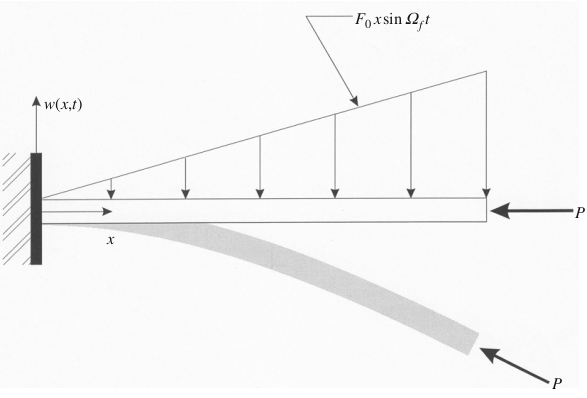
\includegraphics[height=8cm]{fig_2_2}
	\caption{Cantilever beam subjected to a tangential, follower compressive load, $P$ and a time-dependent distributed force, $F(x,t)$}
	\label{fig:forcing}
\end{figure}                   


\subsection{Non-dimensionalization of the equation} The equation \ref{eqn:cantilever-beam-forced} consists of the following physical variables
$$x, L, w, E, I, m, P, F, t, \Omega_f$$
Denoting dimension of mass by $\mathcal{M}$, dimension of length by $\mathcal{M}$ and dimension of time by $\mathcal{T}$, let us construct a time scale as 
$$\sqrt{\frac{mL^4}{EI}} \equiv \sqrt{\frac{\mathcal{ML}^{-1}\mathcal{L}^4}{(\mathcal{M}\mathcal{L}^{-1}\mathcal{T}^{-2})(\mathcal{L}^4)}} = \mathcal{T}$$
Let us non-dimensionalize the variables as

\begin{minipage}{0.5\textwidth}
	\begin{itemize}
		\item $\xi = \frac{x}{L} \equiv \frac{\mathcal{L}}{\mathcal{L}}$
		\item $\eta = \frac{w}{L} \equiv \frac{\mathcal{L}}{\mathcal{L}}$
		\item $\tau = \frac{t}{\sqrt{\frac{mL^4}{EI}}} \equiv \frac{\mathcal{T}}{\mathcal{T}}$
		\item $\mathcal{P} = \frac{PL^2}{EI} \equiv \frac{(\mathcal{M}\mathcal{L}\mathcal{T}^{-2})(\mathcal{L}^2)}{(\mathcal{M}\mathcal{L}^{-1}\mathcal{T}^{-2})(\mathcal{L}^4)}$
		\item $f = \frac{FL^3}{EI} \equiv \frac{(\mathcal{M}\mathcal{T}^{-2})(\mathcal{L}^3)}{(\mathcal{M}\mathcal{L}^{-1}\mathcal{T}^{-2})(\mathcal{L}^4)}$
		\item $\omega_f = \Omega_f\sqrt{\frac{mL^4}{EI}} \equiv \frac{\mathcal{T}}{\mathcal{T}^{-1}}$
	\end{itemize}
\end{minipage}

For the given problem, $F(x,t) = F_0 x \sin (\Omega_f t)$ and its non-dimensional counterpart is 
$$f = \frac{F_0 x \sin (\Omega_f t)~L^3}{EI} = \underbrace{\frac{F_0 L^4}{EI}}_{f_0}\underbrace{\frac{x}{L}}_\xi\sin (\frac{\omega_f}{\sqrt{\frac{mL^4}{EI}}} t) = f_0\xi \sin(\omega_f \tau)$$

Dividing both sides of equation \ref{eqn:cantilever-beam-forced} by $\frac{EI}{L^3}$, we get
\begin{align*}
L^3\pdv[4]{w}{x} + \frac{PL^3}{EI}\pdv[2]{w}{x} + \frac{mL^3}{EI}\pdv[2]{w}{t} &= \frac{F(x,t)L^3}{EI} \\
L^3\pdv[4]{(\eta L)}{(\xi L)} + \frac{PL^3}{EI}\pdv[2]{(\eta L)}{(\xi L)} + \frac{mL^3}{EI}\pdv[2]{(\eta L)}{\left(\sqrt{\frac{mL^4}{EI}}\tau\right) } &= \frac{F(x,t)L^3}{EI} \\
\implies \qquad \pdv[4]{\eta }{\xi} + \mathcal{P}\pdv[2]{\eta}{\xi} + \pdv[2]{\eta }{\tau} &= 0 \\
\implies \qquad \eta^{''''} + \mathcal{P} \eta^{''} + \ddot{\eta} &= f_0\xi \sin(\omega_f \tau) 
\end{align*}
where primes and dots indicate partial differentiation with respect to $\xi$ and $\tau$.

Substituting $\eta (\xi, \tau) \approx \eta_N (\xi, \tau) = \sum_{j=1}^N \phi_j(\xi)q_j(\tau)$ in the above equation, multiplying $\phi (\xi)$ on both sides and integrating from $\xi = 0$ to $\xi = 1$, we get
\begin{align*}
\sum_{j=1}^N\left( \int_0^1 \dv[4]{\phi_j (\xi)}{\xi}\phi_i (\xi) d\xi + \mathcal{P}\int_0^1 \dv[2]{\phi_j (\xi)}{\xi}\phi_i (\xi) d\xi \right) q_j (\tau) &\\
~+ \sum_{j=1}^N\left(\int_0^1 \phi_i(\xi) \phi_j(\xi) d\xi\right) \ddot{q}_j(\tau) &= \int_0^1 f_0\xi \sin(\omega_f \tau) d\xi \\
\sum_{j=1}^N \left(k_{ij} q_j (\tau) + \delta_{ij} \ddot{q}_j(\tau) \right) &= Q_i \sin(\omega_f \tau);~ i=1,2, \cdots, N \\
\implies~\sum_{j=1}^N \left(m_{ij} \ddot{q}_j(\tau) + k_{ij} q_j (\tau)\right) &= Q_i \sin(\omega_f \tau);~ i=1,2, \cdots, N
\end{align*}
where, 
\begin{itemize}
	\item $k_{ij} = \int_0^1 \dv[4]{\phi_j (\xi)}{\xi}\phi_i (\xi) d\xi + \mathcal{P}\int_0^1 \dv[2]{\phi_j (\xi)}{\xi}\phi_i (\xi) d\xi$
	\item $\int_0^1 \phi_i(\xi) \phi_j(\xi) d\xi = \delta_{ij}$
	\item $\int_0^1 \phi_i(\xi) \phi_j(\xi) d\xi = \delta_{ij}, Q_j = \int_0^1 f_0\xi d\xi$
\end{itemize}
We have the following matrix equation
\begin{align}
[I]\{\ddot{q}\} + [K]\{q\} &= \{Q\}\sin(\omega_f \tau) \label{eqn:reduced-matrix-eqn-forced}
\end{align} 
where $[I]$ is the unit matrix
\subsection{Decoupling the equation} As the matrix $[K]$ is asymmetric, we need to resort to biorthogonalization technique to decouple the eqn \ref{eqn:reduced-matrix-eqn-forced}.
Let us determine the eigenvalues, left and right eigenvectors of $[K]$. The right eigenvectors are determined as
\begin{align*}
[K][X] &= [X][\Lambda] 
\end{align*}
where the columns of $[X]$ are the right eigenvectors and $[\Lambda]$ is a diagonal matrix containing the eigenvalues.
The left eigenvectors of $[K]$ are the right eigenvectors of the tranpose of  $[K]$, that is, $[K]^T$
\begin{align*}
[K]^T[Y] &= [Y][\Lambda] \\
\implies [Y]^T[K] &= [\Lambda][Y]^T \quad \text{(tranposing both sides )}
\end{align*}
where the columns of $[Y]$ are the left eigenvectors of $[K]$ and $[\Lambda]$ is the diagonal matrix containing the eigenvalues.
The matrices are orthonormalized such that 
$$[Y]^T[X] = [I]$$
We can express $[K]$ as 
$$[K]=  [Y]^T[\Lambda][X]\quad \text{or } [Y]^T[K][X] = [\Lambda] $$
Introducing a transformation of the form $\{q\} = [X]\{y\}$ in the equation \ref{eqn:reduced-matrix-eqn-forced}, pre-multiplying both sides by $[Y]^T$, we have
\begin{align*}
[I][X]\{\ddot{y}\} + [K][X]\{y\} &= \{Q\}\sin(\omega_f \tau) \\
[Y]^T[X]\{\ddot{y}\} + [Y]^T[K][X]\{y\} &= [Y]^T\{Q\}\sin(\omega_f \tau) \\
\implies \{\ddot{y}\} + [\Lambda]\{y\} &= \{\Psi\}\sin(\omega_f \tau)
\end{align*}
The above equation now reduces to a set of ordinary differential equations or modal equations of the form
\begin{equation}
\ddot{y}_k + \Lambda_k y_k = \Psi_k \sin(\omega_f \tau), \quad k=1,2,\cdots, N \label{eqn:uncoupled-eqn-forced}
\end{equation}
The free response is given by the solution to its homogeneous form, that is,
\begin{equation}
\ddot{y}_k + \Lambda_k y_k = 0, \quad k=1,2,\cdots, N
\end{equation}
is given by $y_k = \alpha_k \cos(\Lambda_k^{1/2}\tau) + \beta_k \sin(\Lambda_k^{1/2}\tau)$ (assuming that $\Lambda_k$ is real) where $\alpha$ and $\beta_k$ are the constants of integration
For forced response, let us assume a solution of the form $y_k = C\sin(\omega_f \tau) + D \cos(\omega_f \tau)$ and put it into the equation \ref{eqn:uncoupled-eqn-forced}
\begin{align*}
-\omega_f^2(C\sin(\omega_f \tau) + D \cos(\omega_f \tau) + \Lambda_k (C\sin(\omega_f \tau) + D \cos(\omega_f \tau)) &= \Psi_k \sin(\omega_f \tau) \\
C(\Lambda_k - \omega_f^2) \sin(\omega_f \tau) + D(\Lambda_k - \omega_f^2) \cos(\omega_f \tau) &= \Psi_k \sin(\omega_f \tau) \\
\implies C = \frac{\Psi_k}{(\Lambda_k - \omega_f^2)}, &\phantom{=}~ D = 0
\end{align*}
Thus, the complete response to eqn \ref{eqn:uncoupled-eqn-forced} is 
$$y_k = \alpha_k \cos(\Lambda_k^{1/2}\tau) + \beta_k \sin(\Lambda_k^{1/2}\tau) + \frac{\Psi_k}{(\Lambda_k - \omega_f^2)}\sin(\omega_f \tau), \quad k=1,2,\cdots,N $$






%\paragraph{Free response} The equation \ref{eqn:matrix-equation} is solved to obtain the free response of the system for a given set of initial conditions.
%Multiply both sides of eqn \ref{eqn:matrix-equation} by $[M]^{-1}$ (assuming $[M]$ is invertible) to get
%\begin{align}
%\{\ddot{q}\} + [W]\{q\} &= \{0\}; \qquad [W] = [M]^{-1}[K] \label{eqn:reduced-matrix-eqn}
%\end{align}
%Let us introduce an oscillatory solution of the form 
%\begin{align*}
%\{q\} &= \{A\}e^{i\Omega t} 
%\end{align*}
%where $\{A\}$ is the column of unknown amplitudes and $\Omega$ the circular frequency
%\begin{align*}
%-\Omega^2\{A\}e^{i\Omega t} + [W]\{A\}e^{i\Omega t} &= \{0\} \\
%\implies \left( [W] - \Omega^2[I]\right) \{A\} &= \{0\}  \qquad [I] \text{ is the identity matrix} 
%\end{align*}
%For non-trivial solution, we must have the following characteristic equation
%$\det([W] - \Omega^2[I]) = 0$
%from which we can obtain $\Omega_i^2,~i=1,2,\cdots, N$ and also their corresponding eigenvectors $\{A\}_i$.
%
%To decouple the equation \ref{eqn:reduced-matrix-eqn}, we introduce the following transformation
%\begin{align}
%\{q\} &= [A]\{y\} \label{eqn:transformation}
%\end{align}
%where the modal matrix, $[A] = [\{A\}_1~\{A\}_2~\cdots~\{A\}_N]$ and $\{y\}$ contains the principal coordinates
%
%Suppose that the eigenvalues are real despite $[K]$ being asymmetric and linearly independent eigenvectors have been found,
%Substituting eqn \ref{eqn:transformation} in \ref{eqn:reduced-matrix-eqn} and pre-multiplying both sides by $[A]^{-1}$, we have
%\begin{align}
%\{\ddot{y}\} &= 
%\end{align}
